\section{Ausblick auf zukünftige Ergänzungen} \label{sec:praktischeUmsetzung:ausblick}

\subsection{Zugriff auf Personendaten und Auswertungen}
Die Auswertung der erbrachten Leistungen einzelner Personen ist aus regulatorischen Gründen ein komplexes Thema und erfordert die Zustimmung des Betriebsrates. Für die meisten Benutzer könnte dies über eine Gruppe mit entsprechenden Rechten im \ac{aad} gelöst werden, in der die Mitglieder vom Betriebsrat verwaltet werden. Datenbankadministratoren hätten jedoch immer noch die Möglichkeit, auf die Personendaten zuzugreifen. 

Mit der Datenbankfunktion \textit{Always Encrypted} kann das verhindert werden. \textit{Always Encrypted} ermöglicht es Spalten zu verschlüsseln und kann damit auch Datenbankadministratoren daran hindern sensitive Daten zu lesen. Der verwendete Schlüssel wird im \textit{Key Vault} gespeichert und die dort eingestellten Zugriffsberechtigungen auf den Schlüssel, bestimmen, wer die Daten unverschlüsselt abfragen kann. Die Entschlüsselung während der Abfrage passiert dabei automatisch \cite{mauri_practical_2021}. Es wäre demnach ausreichend, der zuvor erstellten Gruppe, Zugriff auf den Schlüssel im \textit{Key Vault} zu gewähren. Einem Datenbankadministrator, der nicht in dieser Gruppe ist, werden dann nur verschlüsselte Binärwerte angezeigt und er kann keine Auswertungen durchführen.

\subsection{Machine Learning für fortgeschrittene Analysen}
\label{sec:praktischeUmsetzung:ausblick:aml}
Die Einbindung von \ac{aml} ist komplexer als ursprünglich erwartet. Das liegt zum einen an der Abhängigkeit zu zusätzlichen Diensten und zum anderen an der Anforderung, diese Dienste in einer sicheren Umgebung zu betreiben. Abbildung~\ref{fig:praktischeUmsetzung:ausblick:aml} zeigt ein vereinfachtes Konzept, noch ohne die Berücksichtigung eines sicheren Netzwerks, wie die Ergänzung von \ac{aml} zukünftig aussehen könnte.

\begin{figure}[htbp]
 \centering
 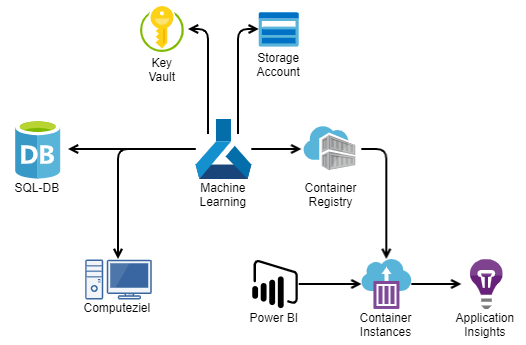
\includegraphics[width=\textwidth]{gfx/aml.png}
 \caption[Konzept: Azure Machine Learning]{Vereinfachtes Konzept zur zukünftigen Verwendung von Azure Machine Learning \cite[vgl.][]{msdoc_22_aml_arch}}
\label{fig:praktischeUmsetzung:ausblick:aml}
\end{figure}

Das Konzept soll stichpunktartig beschrieben werden \cite[vgl.][]{msdoc_22_aml_arch, soh_data_2020}:
\begin{itemize}
\item Benutzer erstellen mit \ac{aml} neue Modelle mit Python oder R.
\begin{itemize}
    \item Die auf Daten aus dem \ac{dwh}, werden dabei als Dataset leicht zugänglich gemacht.
    \item Das Training geschieht auf einem beliebigen Computeziel. Zum Beispiel dem lokalen Rechner, einer \ac{vm} oder einem Cluster aus mehreren Rechnern.
    \item Metadaten und Skripte werden in einem Storage Account gespeichert.
    \item Für Zugriffsdaten wird der Key Vault verwendet.
\end{itemize}
\item Mit dem Modell und allen Abhängigkeiten wird ein Docker-Image erstellt, welches in der Container Registry gespeichert wird.
\item Das Docker-Image wird mit Container Instances (oder alternativ mit Azure Kubernetes Services) als Web Services zur Verfügung gestellt.
\item Power BI kann auf den Webservice aufrufen und die Ergebnisse in Reports verwenden.
\item Monitorinformationen über das Modell und den Webservice werden mit Application Insights gesammelt und gespeichert.
\end{itemize}

Bereits diese vereinfachte Darstellung zeigt, dass die Ergänzung von \ac{aml} deutlich komplexer als bei anderen Diensten ist. Es sollte hinterfragt werden, ob es die richtige Entscheidung war, Azure SQL Database und \ac{aml} in Abschnitt~\ref{sec:konzeption:evaAuswertung} auszuwählen. Mit der SQL Managed Instance könnten ohne zusätzliche Infrastruktur die \textit{SQL Server Machine Learning Services} verwendet werden und somit Python und R Skripte ausgeführt werden. Hier sind die Möglichkeiten jedoch deutlich eingeschränkter und es stehen nur wenige Algorithmen zur Auswahl \cite{etaati_introduction_2019}. Daher ist es für eine optimale Umsetzung unumgänglich, eine spezifischere Analyse und Beschreibung der Anforderung vorzunehmen. Insgesamt kann festgehalten werden, dass zukünftig weitere Untersuchungs- und Evaluationszeit für die fortgeschrittenen Analysen eingeplant werden sollte.